\documentclass[12pt]{article}
\usepackage[utf8]{inputenc}
\usepackage[russian]{babel}
\usepackage [left=30 mm, top=30 mm, right=30 mm, bottom=20mm, nohead, footskip=10 mm] {geometry}
%\usepackage{pscyr}
\usepackage[T2A]{fontenc}
\usepackage{amsmath}
\usepackage{amssymb}
\usepackage{graphicx}
\graphicspath{{src/}}
\usepackage{listings}   
\usepackage{hyperref}
\usepackage{fancyhdr}
%\usepackage{algorithm}
\usepackage{algpseudocode}
\usepackage{indentfirst}
\usepackage{listings}
\usepackage{caption}
\usepackage{hyperref}
\addto\captionsrussian{\def\refname{Список источников}}
\hypersetup{
    colorlinks=true,
    linkcolor=blue,
    filecolor=magenta,      
    urlcolor=cyan,
}
\usepackage{float}%"Плавающие" картинки
\hypersetup{
    colorlinks=true,
    linkcolor=blue,
    filecolor=magenta,      
    urlcolor=cyan,
    pdftitle={Sharelatex Example},
    bookmarks=true,
    pdfpagemode=FullScreen,
}
\usepackage{wrapfig}%Обтекание фигур (таблиц, картинок и прочего)

\parindent=24pt

\begin{document}

\begin{center}
\hfill \break
\large{МИНОБРНАУКИ РОССИИ} \\
\hfill \break
\small {ФЕДЕРАЛЬНОЕ ГОСУДАРСТВЕННОЕ БЮДЖЕТНОЕ ОБРАЗОВАТЕЛЬНОЕ УЧРЕЖДЕНИЕ }\\
\small { ВЫСШЕГО ПРОФЕССИОНАЛЬНОГО ОБРАЗОВАНИЯ  } \\
\hfill \break
\normalsize {\textbf{ <<САНКТ-ПЕТЕРБУРГСКИЙ ПОЛИТЕХНИЧЕСКИЙ УНИВЕРСИТЕТ } }\\
{\normalsize {\textbf { ПЕТРА ВЕЛИКОГО>>}}} \\
\hfill \break
\large{Институт Компьютерных Наук и Кибербезопасности }\\
\hfill \break
\large{ Высшая школа технологий искуственного интелекта }\\
\hfill \break
Направление 02.03.01 Математика и Компьютерные Науки\\
\vskip 1cm
\large {Отчет по лабораторной работе №2.}
\vskip 0.2cm
\large {По дисциплине:}

\large{<<Алгоритмические основы компьютерной графики>>} \\
\hfill \break
\normalsize{Тема Работы:} \\
\hfill \break
\normalsize{<<Изучение алгоритма Вейлера-Азертона>>} \\
\thispagestyle {empty}

\hfill \break
\vskip 0.3cm
\vskip 1cm
\end{center}
\begin {tabular}{cccc}
\hspace{0.5cm}Обучающийся: &\underline {\hspace{3cm}} &  &Черепанов Михаил Дмитриевич\\\\
\hspace{0.5cm}Руководитель: &\underline {\hspace{3cm}} & &Курочкин Михаил Александрович\\\\
\end{tabular}
\vskip 0.5 cm
\hspace{9cm}\def \hrf#1{\hbox to#1{\hrulefill}}<<\hrf{2em}>>  \hrf{6em}  20\hrf{1em}~r.
\vskip 2cm
\begin {center} Санкт-Петербург 2024 \end{center}
\newpage
\tableofcontents
\newpage




\section*{Введение}
 \addcontentsline{toc}{section}{Введение}
 sasasas
 
 Компьютерная (машинная) графика — это совокупность методов и приемов для преобразования при
помощи компьютера данных в графическое представление.
Таким образом, машинная графика представляет собой комплекс аппаратных и программных средств
для создания, хранения, обработки и наглядного представления графической информации с помощью
компьютера.

Алгоритмы в компьютерной графике используются для решения задач построения геометрического
объекта, геометрических преобразований (поворот, перенос, изменение масштаба и др.), позиционирования (определение линий пересечения поверхностей), метрических операций (вычисление длины линии,
площади поверхности, объёма, тела и др.).


 Одной из фундаментальных задач компьютерной графики является отсечение многоугольников.


Отсечение многоугольников в компьютерной графике — это процесс определения видимых частей многоугольников, которые должны быть отображены на экране, и исключения невидимых частей, которые находятся за пределами определённой области видимости или за границами экрана.

В данной лабораторной работе предлагается изучить и реализовать один из наиболее часто используемых алгоритмов отсечения многоугольников - алгоритм Вейлера-Азертона.



\newpage

\section{Описание алгоритма Вейлера-Азертона}

Алогритм Вейлера-Азертона позволяет производить отсечение невыпуклого многоугольника с внутренними
отверстиями по другому невыпуклому многоугольнику, который
также имеет внутренние отверстия. Будем называть многоугольник, который отсекается, обрабатываемым многоугольником, а
многоугольник, по которому производится отсечение, — отсекающим
многоугольником
(отсекателем).
 
Сложность данного алгоритма - O($ N^2 $), где N - суммарное количество вершин в обоих многоугольниках.





Итак, обобщим:

{ \bf Входные данные алгоритма:}

Два многоугольника(обрабатываемый и отсекающий), возможно с внутренними отверстиями.

Оба многоугольника могут быть как выпуклыми, так и невыпуклыми.

Каждый из многоугольников представлен ввиде набора циклических списков вершин.


Если многоугольник состоит из нескольких контуров, то каждый из контуров подается отдельным циклическим списком. 

{ \bf Выходные данные алгоритма:}

Многоугольник, полученный в результате отсечения от обрабатываемого многоугольника области, ограниченной отсекателем.

Выходной многоугольник так же представлен одним (или более) списком вершин.

В случае, если области обрабатываемого и отсекающего многоугольников не перекрываются - выводится пустой список вершин.

{ \bf Ограничения:}

Контуры входных многоугольников не должны иметь самопересечений.

Ориентация вершин в циклических списках для внешних контуров должна быть по часовой стрелке.
Для внутренних - против часовой.

Алгоритм работает только с двухмерными многоугольниками.






\newpage
\section{Постановка задачи}

1. Изучить алгоритм Вейлера-Азертона.

2. Программно реализовать данный алгоритм.

3. Сравнить свою реализацию с имеющейся библиотечной по времени работы  при равных условиях.

\newpage



\section{Описание алгоритма}


Как уже было сказано, на вход алгоритма подаются два многоугольника - обрабатываемый и отсекающий - в виде циклических списков вершин.  В каждом элементе списка лежит пара (x,y)  координат вершин и указатель на следующую вершину многоугольника.

 Границы обрабатываемого и отсекающего многоугольников могут
пересекаться или не пересекаться между собой. Если они пересекаются, то точки пересечения образуют
пары. Одно пересечение из пары возникает, когда ребро обрабатываемого многоугольника входит внутрь
отсекающего многоугольника, а другое — когда оно выходит оттуда. Основная идея заключается в том,
что алгоритм начинает с точки пересечения входного типа, затем он прослеживает внешнюю границу по
часовой стрелке до тех пор, пока не обнаруживается еше одно ее пересечение с отсекающим многоугольников. В точке последнего пересечения производится поворот направо и далее прослеживается внешняя
граница отсекателя по часовой стрелке до тех пор, пока не обнаруживается се пересечение с обрабатываемым многоугольником. И вновь в точке последнего пересечения производится поворот направо и далее прослеживается граница обрабатываемого многоугольника. Этот процесс продолжается до тех пор, пока не встретится начальная вершина. Внешние границы многоугольника обходятся по часовой стрелки ,  внутренние границы против часовой стрелки.




Более формальная запись этого алгоритма имеет следующий вид:



\begin{enumerate}
\item Вычислить все пересечения обрабатываемого и отсекающего многоугольников.
\begin{enumerate}
\item Добавить все эти пересечения к спискам вершин обрабатываемого и отсекаюшего многоуголь
ников.

\item Пометить все точки пересечения и установить двусторонние связи между списками вершин
обрабатываемого и отсекающего многоугольников для каждой такой точки.






\end{enumerate}






\item   Обработать непересекаюшиеся границы многоугольников.
\begin{enumerate}
\item Установить два списка принадлежности, один для границ обрабатываемого многоугольника, лежащих внутри отсекателя	, и другой для границ, лежаших вне отсекателя. Проигнорировать такие
границы отсекателя, которые лежат вне обрабатываюшего многоугольника.

\item  Границы отсекателя, попавшие внутрь обрабатывающего многоугольника, образуют н нем дыры. Следовательно, копии границ отсекающего многоуголыника должны попасть в оба списка
принадлежности: внутренний и внешний. Занести эти границы в соответствующие списки принадлежности.
\end{enumerate}







\item  Создать два списка вершин, являющихся точками пересечения.
\begin{enumerate}
\item Один — список входов — содержит только пересечения, образованные ребрами обрабатываемого
многоугольника, которые входит внутрь отсекателя.

\item Другой список выходов — содержит только пересечения, образованные ребрами обрабатываемого многоугольника, которые выходят изнутри отсекателя. Типы точек пересечения будут
чередоваться при обходе границы. Поэтому достаточно определить тип только у одной из каж-
дой пары точек пересечения.








\end{enumerate}

\item Реализовать отсечение

Поиск многоугольников, лежащих внутри отсекателя, ведется с помощью следующей процедуры:

\begin{enumerate}
\item Взять точку пересечения из списка входов. Если этот список пуст, то поиск завершен.


\item Просматривать список вершин обрабатываемого многоугольника, начиная с текущего пересечения,  до тех пор, пока не обнаружится следующее пересечение.

Скопировать вершины из списка вершин обрабатываемого многоугольника вплоть до этого
пересечения в список внутренней принадлежности (Пересечение включается) .


\item Используя двустороннюю связь,перейти к списку вершин отсекающего многоугольника.

\item Просматривать список вершин отсекателя, начиная с текущего пересечения,  до тех пор, пока не обнаружится следующее пересечение.

Скопировать вершины из списка вершин отсекателя вплоть до этого пересечения в список
внутренней принадлежности.

\item Вернуться назад в список вершин обрабатываемого многоугольника(Пересечение включается).

\item Повторять эти действия по тех пор, пока не будет достигнута начальная вершина. В этот
момент новый внутренний многоугольник замыкается.

\end{enumerate}

Поиск многоугольников, лежащих вне отсекателя ведется с помощью такой же процедуры, за исключением того, что начальная точка пересечения берется из списка выходов, а вершины из
списка вершин отсекателя просматриваются в обратном порядке. Списки вершин многоугольников при этом копируются в список внешней принадлежности.
\item Связать все отверстия, т. е. внутренние границы, с соответствующими им внешними границами.
Поскольку внешние границы ориентированы по часовой стрелке, а внутренние границы — против
часовой стрелки, эту операцию удобно выполнить путем проверки ориентации границ.


\item  Процесс завершен.




\end{enumerate}

\newpage
\section{Описание реализованной программы}

Для реализации данного алгоритма был выбран язык java и Среда разработки IntelliJ IDEA.

Программа содержит следующие классы:
\begin{enumerate}
\item { \bf Main}: исполняемый класс, в котором программа:

1. Запрашивает у пользователя последовательный ввод точек каждого из многоугольников.

2. Производит проверку на то, что грани многоугольников взаимонепересекающиеся.

3. Вызов метода GetIntersection класса WeilerAtherton(описан далее) для получения результа.

4. Вывод на экран результата работы программы.


\item { \bf Point}: класс, в котором хранятся координаты точек многоугольников. Объекты класса являются элементами связных циклических списков.


\item { \bf Polygon}: класс реализующий многоугольник набором связных циклических списков.

\item { \bf WeilerAtherton}: Класс, реализующий алгоритм Вейлера-Азертона.

Основные методы класса:

\begin{enumerate}
\item { \bf ComputeIntersections}

Входные данные:

2 объекта класса Polygon: обрабатываемый и отсекащий многоугольники. 

Выходные данные: 

2 объекта класса Polygon: обрабатываемый и отсекащий многоугольники, к каждому из которых добавлены точки их пересечения.



\item { \bf processNonIntersectingEdges}

Входные данные:

2 объекта класса Polygon: обрабатываемый и отсекащий многоугольники. 

Выходные данные:
 Два списка принадлежности (Внутренний и внешний).


\item { \bf PerformClipping}

Входные данные:

2 объекта класса Polygon: обрабатываемый и отсекащий многоугольники, внутренний и внешний списки принадлежности.

Выходные данные: 
Объект класса Polygon, представляющий собой результирующий многоугольник.

\item { \bf GetIntersection}


Входные данные:

2 объекта класса Polygon: обрабатываемый и отсекащий многоугольники.

Выходные данные: 
Объект класса Polygon, представляющий собой результирующий многоугольник.


В данном методе последовательно вызываются вышеописанные функции для получения финального результата.


\end{enumerate}

 
\end{enumerate}




Исходный код программы представлен в приложении 1.









\section{Сравнение с библиотечной реализацией}


Для сравнения с реализованным алгоритмом была выбрана библиотека JTS Topology Suite (JTS).

JTS Topology Suite (JTS) - это программная библиотека Java с открытым исходным кодом, которая предоставляет объектную модель для плоской геометрии вместе с набором фундаментальных геометрических функций. 



Данная библиотека содержит следующие функции и структуры:  

геометрические модели (точка, линия, полигон);

геометрические операции (пересечение, объединение, нахождение внутри, и т.д.).

Из данной библиотеки был взят метод Intersection (класс Geometry), в основе которого лежит алгоритм Вейлера-Азертона.



Результаты работы программы:

На рис. \ref{fig:i0} ,  \ref{fig:i3}, \ref{fig:i7} показаны примеры входных данных для обработки алгоритмом.

На рис. \ref{fig:i1} , \ref{fig:i4}, \ref{fig:i8} показаны результаты работы алгоритма моей реализации.

На рис. \ref{fig:i2} ,  \ref{fig:i6} , \ref{fig:i9} показаны результаты работы библиотечного алгоритма. 



На рисунках красным цветом обозначен обрабатываемый многоугольник. Зеленым - отсекающий. Синим - результирующий многоугольник.

Пример №1:

\vskip 1cm
{
    \centering
    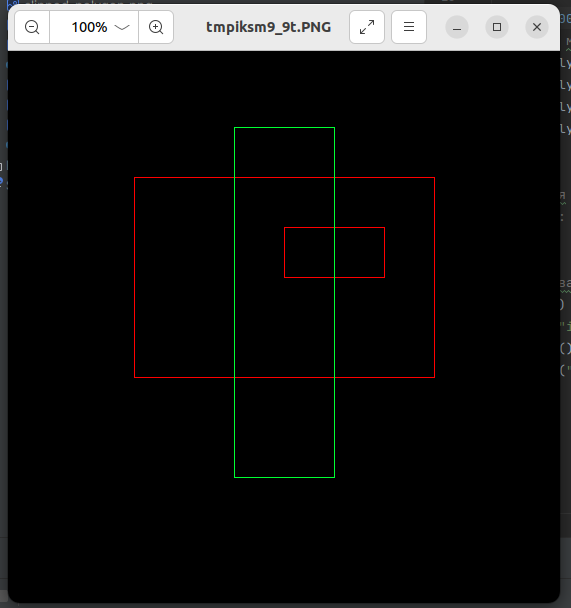
\includegraphics[width=0.5\linewidth]{вход1.png}
    \captionof{figure}[]{Входные данные 1.}
    \label{fig:i0}
}
\vskip 1cm


\vskip 1cm
{
    \centering
    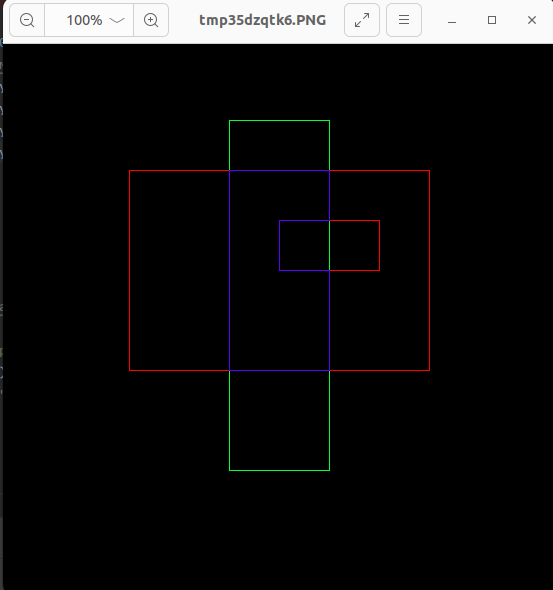
\includegraphics[width=0.5\linewidth]{резмой1.png}
    \captionof{figure}[]{Результат работы моей реализации 1}
    \label{fig:i1}
}
\vskip 1cm




\vskip 1cm
{
    \centering
    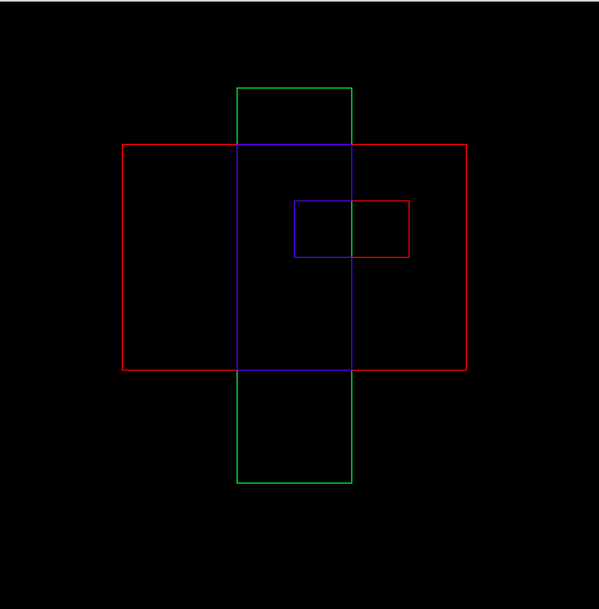
\includegraphics[width=0.5\linewidth]{рез1_биб.png}
    \captionof{figure}[]{Результат работы библиотечного алгоритма 1}
    \label{fig:i2}
}
\vskip 1cm


Пример №2:
\vskip 1cm
{
    \centering
    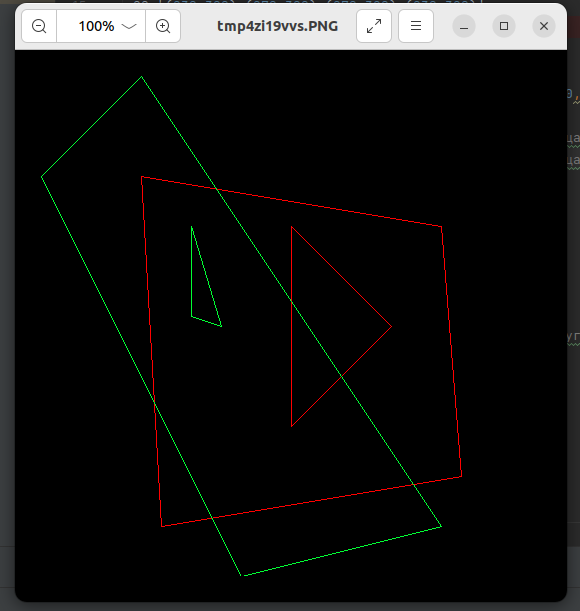
\includegraphics[width=0.5\linewidth]{вход2.png}
    \captionof{figure}[]{Входные данные 2.}
    \label{fig:i3}
}
\vskip 1cm


\vskip 1cm
{
    \centering
    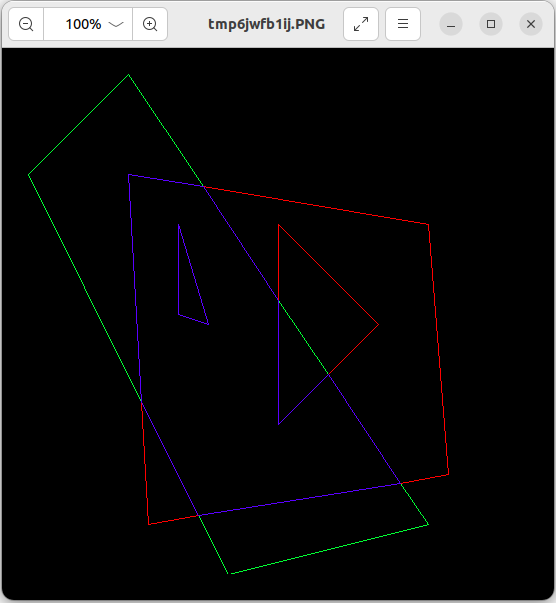
\includegraphics[width=0.5\linewidth]{резмой2.png}
    \captionof{figure}[]{Результат работы моей реализации 2}
    \label{fig:i4}
}
\vskip 1cm


\vskip 1cm
{
    \centering
    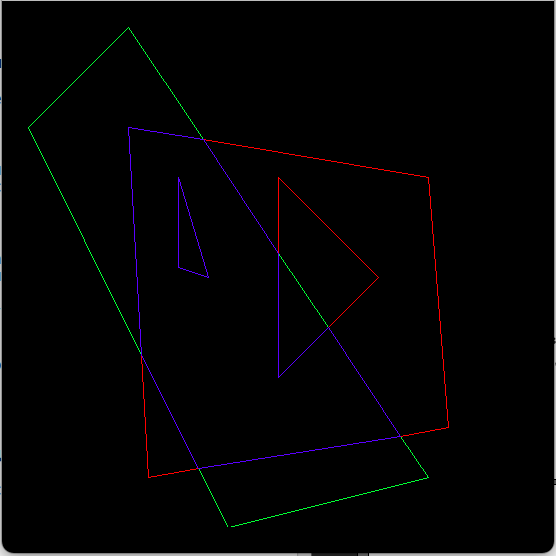
\includegraphics[width=0.5\linewidth]{рез2_биб.png}
    \captionof{figure}[]{Результат работы библиотечного алгоритма 2}
    \label{fig:i6}
}
\vskip 1cm

Пример №3:

\vskip 1cm
{
    \centering
    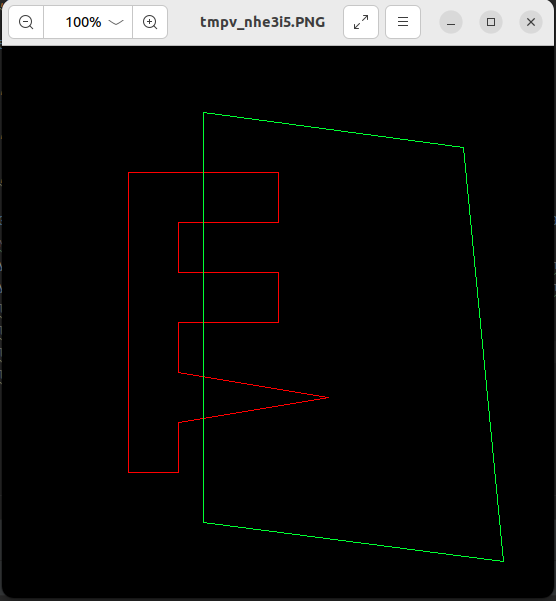
\includegraphics[width=0.5\linewidth]{вход3.png}
    \captionof{figure}[]{Входные данные 3.}
    \label{fig:i7}
}
\vskip 1cm


\vskip 1cm
{
    \centering
    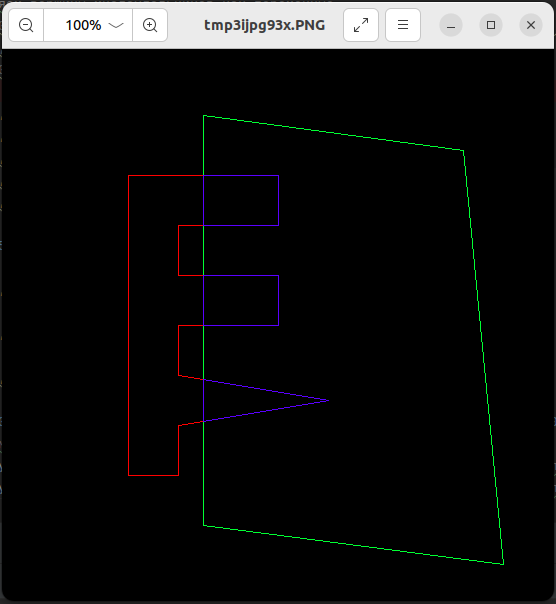
\includegraphics[width=0.5\linewidth]{резмой3.png}
    \captionof{figure}[]{Результат работы моей реализации 3}
    \label{fig:i8}
}
\vskip 1cm


\vskip 1cm
{
    \centering
    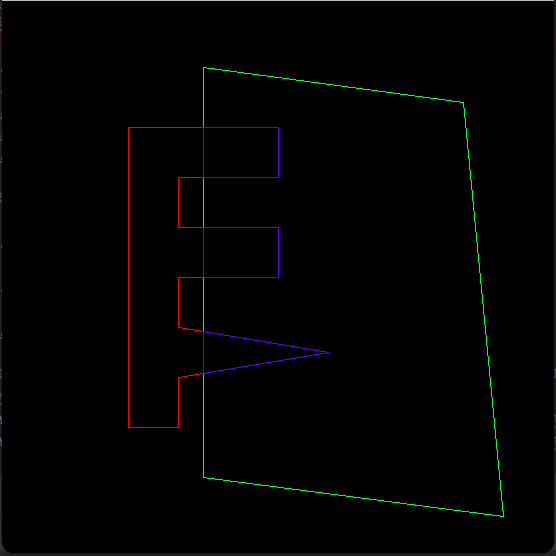
\includegraphics[width=0.5\linewidth]{рез3_биб.png}
    \captionof{figure}[]{Результат работы библиотечного алгоритма 3}
    \label{fig:i9}
}
\vskip 1cm





Как видно из представленных примеров при одинаковых входных данных, выходные данные моей и библиотечной реализаций совпадают(в том числе, в случае получении в результате отсечения нескольких многоугольников).




\subsection{Проведение эксперимента}

Эксперимент для сравнения эффективности работы самостоятельно реализованного алгоритма проводился на компьютере с процессором Intel Core i7 с частотой 2.40 гГц. В эксперименте исследуется
время, затраченное на проведение отсечения многоугольников реализованным и библиотечным методами.

Эксперимент заключается в том, что сначала пользователь вводит координаты обрабатываемого многоугольника и отсекателя, а затем отсекатель начинает смещаться вниз на 1 по координате Х. После
каждого смещения происходит нахождение пересечения реализованным методом и библиотечным, а затем вычисляется затраченное время. Всего происходит n смещений. В экспериментах количество смещений (число n)
изменяется от 5 до 1000.

Для сравнения времени, затраченного реализованным алгоритмом и библиотечным, был выбран метод
System.nanoTime(). Метод возвращает текущее значение наиболее точного доступного системного таймера
в наносекундах. Возвращаемое значение представляет наносекунды с некоторого фиксированного момента
времени.

При проведении эксперимента замеряется только время, которое было затрачено на отсечение, при
этом реализованный и библиотечный методы вызываются по очереди, поэтому реализации поставлены в
одинаковые условия. Итоговое время вычисляется как сумма промежуточных измерений.




В таблице ниже представлены результаты проведённого эксперимента. В данной таблице указано время в
наносекундах, затраченное  на пересечение многоугольников, при n смещениях отсекателя.

Для проведения эксперимента использовались многоугольники из примера №2.


\vskip 1cm
{
    \centering
    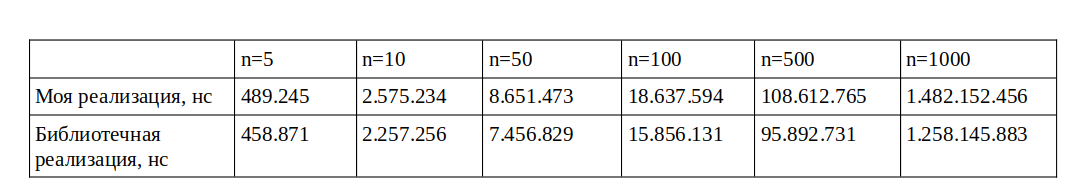
\includegraphics[width=1\linewidth]{результаты.png}

    \label{fig:i5}
}
\vskip 1cm


В ходе эксперимента выяснилось, что время работы моей реализации сопоставимо со временем работы библиотечного алгоритма.

На полученную оценку могут влиять задачи, которые процессор выполняет параллельно.

 \newpage
 
 \section{Заключение}
 
 В ходе выполнения работы было сделано:
 
 1. Изучен и программно реализован алгоритм отсечения многоугольников Вейлера-Азертона.
 
 2. Данная реализация была сравнена с библиотечной. В ходе сравнения выяснилось, что данная реализация сопостовима по времени работы с библиотечной.
 
 














 \addcontentsline{toc}{section}{Список использованных источников}
 \newpage
\renewcommand{\refname}{Список использованных источников}
\begin{thebibliography}{99}

  

    \bibitem{source2}  {Алгоритмические основы машинной графики.
Д. Роджерс. Москва <<Мир>> 1989 г.}
    
     

\end{thebibliography}


 \newpage
 
 {\bf \LARGE Приложение 1.}












\textbf{Код программы:}




 \vskip 1 cm
 \medskip
\hrule width 16cm height 1pt

\lstset{language=Python}          % Задаем язык исходного кода
\begin{lstlisting}  

public class Main {
    public static void main(String[] args) {
        Scanner scanner = new Scanner(System.in);


        Polygon polygon = new Polygon();
        System.out.println("Enter coordinates:");
        int x, y;
        while (true) {
            System.out.print("Enter x coordinate:");
            x = scanner.nextInt();
            if (x == -1) break;
            System.out.print("Enter y coordinate:");
            y = scanner.nextInt();
            polygon.addPoint(x, y);
        }


        Polygon clipper = new Polygon();
        System.out.println("Enter coordinates:");
        while (true) {
            System.out.print("Enter x coordinates:");
            x = scanner.nextInt();
            if (x == -1) break;
            System.out.print("Enter y coordinate:");
            y = scanner.nextInt();
            clipper.addPoint(x, y);
        }

     
        System.out.println("Polygon:");
        polygon.printPolygon();
        System.out.println("Clipper:");
        clipper.printPolygon();
    }
}











package org.example;

class Point {
    int x, y;
    Point next;

    public Point(int x, int y) {
        this.x = x;
        this.y = y;
        this.next = null;
    }
}










package org.example;

class Polygon {
    Point[] contours;

    public Polygon(int numContours) {
        this.contours = new Point[numContours];
    }

    public void addPoint(int
     contourIndex, int x, int y) {
        Point newPoint = new Point(x, y);
        if (contours[contourIndex] == null) {
            contours[contourIndex] = newPoint;
            contours[contourIndex].next = newPoint; // make it cyclic
        } else {
            Point temp = contours[contourIndex];
            while (temp.next != contours[contourIndex]) {
                temp = temp.next;
            }
            temp.next = newPoint;
            newPoint.next = contours[contourIndex]; // make it cyclic
        }
    }

    public void printPolygon() {
        for (int i = 0; i < contours.length; i++) {
            System.out.println("Contour " + (i + 1) + ":");
            if (contours[i] == null) {
                System.out.println("Empty contour");
                continue;
            }
            Point temp = contours[i];
            do {
                System.out.println("(" + temp.x + ", " + temp.y + ")");
                temp = temp.next;
            } while (temp != contours[i]);
        }
    }
}











package org.example;

import java.util.ArrayList;
import java.util.List;

public class WeilerAtherton {
    Polygon P1;
    Polygon P2;


    public void ComputeIntersections(Polygon
     subjectPolygon, Polygon clipPolygon) {
        List<Point> subjectIntersections = new ArrayList<>();
        List<Point> clipIntersections = new ArrayList<>();

          
        for (int i = 0; i < subjectPolygon.contours.size(); i++) {
            Point[] subjectContour = subjectPolygon.contours.get(i);
            for (int j = 0; j < subjectContour.length; j++) {
                Point p1 = subjectContour[j];
                Point p2 = subjectContour[(j + 1) % subjectContour.length];

                for (int k = 0; k < clipPolygon.contours.size(); k++) {
                    Point[] clipContour = clipPolygon.contours.get(k);
                    for (int l = 0; l < clipContour.length; l++) {
                        Point q1 = 
                        clipContour[l];
                        Point q2 =
                         clipContour[(l + 1) % clipContour.length];

                        Point intersection =
                         getIntersection(p1, p2, q1, q2);
                        if (intersection != null) {
                            subjectIntersections.
                            add(intersection);
                            clipIntersections.
                            add(intersection);
                        }
                    }
                }
            }
        }

   
        for (Point intersection : subjectIntersections) {
            subjectPolygon.addIntersection
            (intersection);
        }
        for (Point intersection : clipIntersections) {
            clipPolygon.addIntersection
            (intersection);
        }
 
        for (Point intersection : subjectIntersections) {
            intersection.nextInSubject =
             findNextIntersection(intersection, subjectPolygon);
            intersection.prevInSubject =
             findPrevIntersection(intersection, subjectPolygon);
        }
        for (Point intersection : clipIntersections) {
            intersection.nextInClip =
             findNextIntersection(intersection, clipPolygon);
            intersection.prevInClip =
             findPrevIntersection(intersection, clipPolygon);
        }
    }


    private boolean isInsidePolygon
    (Point point, Polygon polygon) {
        boolean inside = false;
        for (Point[] contour :
         polygon.contours) {
            for (int i = 0, j = 
            contour.length - 1; i < contour.length; j = i++) {
                if ((contour[i].y
                 > point.y) 
                 != (contour[j].y > point.y) &&
                        (point.x 
                        < (contour[j].x - contour[i].x) * 
                        (point.y - contour[i].y) / (contour[j].y -
                         contour[i].y) + contour[i].x)) {
                    inside = !inside;
                }
            }
        }
        return inside;
    }

    private boolean 
    isOutsidePolygon(Point point, Polygon polygon) {
        return !isInsidePolygon(point, polygon);
    }

    public void processNonIntersectingEdges
    (Polygon subjectPolygon, Polygon clipPolygon) {
        List<Edge> insideSubjectEdges =
         new ArrayList<>();
        List<Edge> outsideSubjectEdges =
         new ArrayList<>();

        
        for (int i = 0; i < subjectPolygon.contours.size(); i++) {
            Point[] subjectContour =
         subjectPolygon.contours.get(i);
            for (int j = 0; j < subjectContour.length; j++) {
                Point p1 = subjectContour[j];
                Point p2 = subjectContour[(j + 1) % subjectContour.length];
                Edge edge = new Edge(p1, p2);

                boolean insideClip =
                 isInsidePolygon(p1, 
                 clipPolygon);
                boolean outsideClip =
                 isOutsidePolygon(p1, clipPolygon);
                if (insideClip && !outsideClip) {
                    insideSubjectEdges.add(edge);
                } else if (!insideClip && outsideClip) {
                    outsideSubjectEdges.add(edge);
                }
            }
        }

        ,    ,    
        for (int i = 0; i < clipPolygon.contours.size(); i++) {
            Point[] clipContour = clipPolygon.contours.get(i);
            for (int j = 0; j < clipContour.length; j++) {
                Point p1 = clipContour[j];
                Point p2 = clipContour[(j + 1) % clipContour.length];
                Edge edge = new Edge(p1, p2);

                boolean insideSubject = isInsidePolygon(p1, subjectPolygon);
                if (insideSubject) {
                    insideSubjectEdges.add(edge);
                    outsideSubjectEdges.add(edge);
                }
            }
        }


        List<Point> entries =
         findIntersections
         (insideSubjectEdges, outsideSubjectEdges);
        List<Point> exits =
         findIntersections(outsideSubjectEdges, insideSubjectEdges);

        
        System.out.println("Entries:");
        for (Point entry : entries) {
            System.out.println("(" 
            + entry.x + ", " + entry.y + ")");
        }

        System.out.println("Exits:");
        for (Point exit : exits) {
            System.out.println("(" 
            + exit.x + ", " + exit.y + ")");
        }
    }

    private List<Point> findIntersections(List<Edge> edges1, 
    List<Edge> edges2) {
        List<Point> intersections =
         new ArrayList<>();
        for (Edge edge : edges1) {
            if (edges2.contains(edge)) {
                intersections.add(edge.start);
            }
        }
        return intersections;
    }



    public void PerformClipping(Polygon
    
     subjectPolygon, Polygon clipPolygon) {
        List<Polygon> clippedPolygons = new ArrayList<>();

       
        for (Point entry : subjectPolygon.entries) {
            List<Point> innerPoints = new ArrayList<>();
            innerPoints.add(entry);

            
            Point currentPoint = entry;
            while (!subjectPolygon.exits.contains(currentPoint)) {
                currentPoint = currentPoint.nextInSubject;
                innerPoints.add(currentPoint);
            }

       
            currentPoint = currentPoint.nextInClip;

                
            while (!clipPolygon.exits.contains(currentPoint)) {
                innerPoints.add(currentPoint);
                currentPoint = currentPoint.nextInClip;
            }

         
            currentPoint = currentPoint.nextInSubject;

     
            while (!entry.equals(currentPoint)) {
                innerPoints.add(currentPoint);
                currentPoint = currentPoint.nextInSubject;
            }

              
            clippedPolygons.add(new Polygon(innerPoints));
        }

        
        System.out.println("Clipped Polygons:");
        
        for (Polygon clippedPolygon : clippedPolygons) {
            for (Point point : clippedPolygon.points) {
                System.out.println("("
                 + point.x + ", " + point.y + ")");
            }
            System.out.println();
        }
    }


    public Polygon getIntersection(Polygon
     subjectPolygon, Polygon clipPolygon) {
        Polygon intersection;

       

        return intersection;
    }

}


























\end{lstlisting}  
\medskip
\hrule width 16cm height 1pt
\bigskip

















\end{document}